\documentclass[tikz,border=7pt]{standalone}
\usepackage[T1]{fontenc}
\usepackage{helvet}
\usepackage{amsmath,amssymb}
\renewcommand{\familydefault}{\sfdefault}
\usetikzlibrary{arrows.meta,positioning,fit,calc,backgrounds}

\definecolor{navy}{HTML}{17324D}
\definecolor{blue}{HTML}{2F6B9A}
\definecolor{cyan}{HTML}{DCEFF5}
\definecolor{teal}{HTML}{278C82}
\definecolor{green}{HTML}{DFF2E7}
\definecolor{orange}{HTML}{E58B3A}
\definecolor{gold}{HTML}{F8E6B6}
\definecolor{purple}{HTML}{7457A6}
\definecolor{lavender}{HTML}{E9E2F5}
\definecolor{ink}{HTML}{263442}
\definecolor{muted}{HTML}{607385}
\definecolor{panel}{HTML}{F6F8FA}
\newcommand{\dimtext}{\scriptsize\color{muted}}

\begin{document}
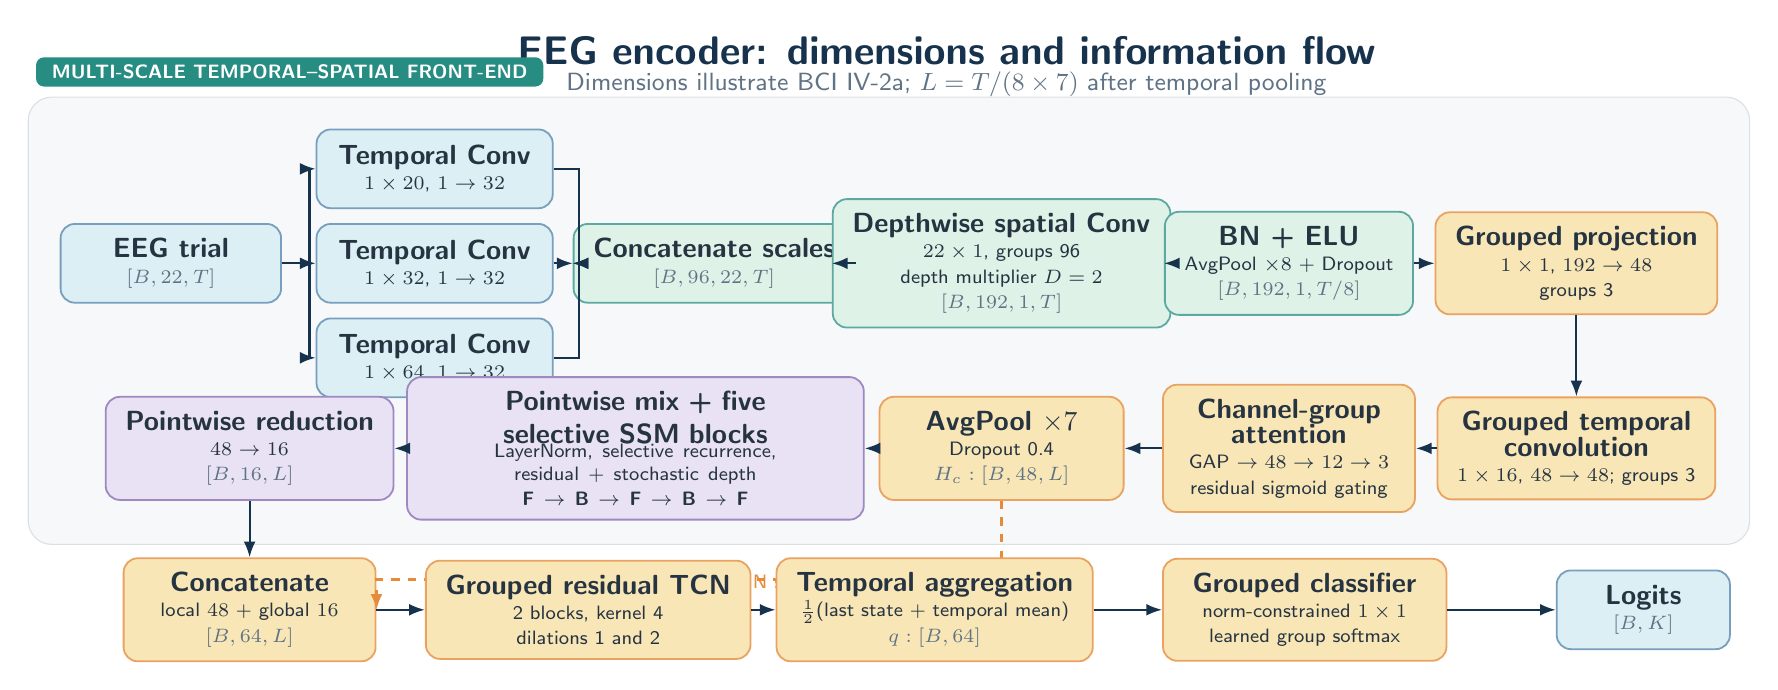
\begin{tikzpicture}[
  font=\sffamily,
  >=Latex,
  flow/.style={-{Latex[length=2mm]}, line width=0.78pt, draw=navy},
  skip/.style={-{Latex[length=2mm]}, line width=0.78pt, draw=orange, dashed},
  card/.style={rounded corners=1.8mm, minimum height=10mm, minimum width=2.55cm,
               align=center, draw=navy!35, line width=0.65pt, fill=white,
               text=ink, inner xsep=2.5mm, inner ysep=1.8mm},
  temporal/.style={card, fill=cyan, draw=blue!65},
  spatial/.style={card, fill=green, draw=teal!75},
  state/.style={card, fill=lavender, draw=purple!70},
  refine/.style={card, fill=gold, draw=orange!80},
  annotation/.style={font=\scriptsize, text=muted},
  heading/.style={font=\bfseries\small, text=navy},
  tag/.style={font=\bfseries\scriptsize, text=white, rounded corners=1mm,
              inner xsep=2mm, inner ysep=1mm}
]

\node[font=\bfseries\Large, text=navy] at (11.2,8.05)
  {EEG encoder: dimensions and information flow};
\node[font=\small, text=muted] at (11.2,7.62)
  {Dimensions illustrate BCI IV-2a; $L=T/(8\times7)$ after temporal pooling};

% input and branches
\node[temporal, minimum width=2.8cm] (input) at (1.35,5.35) {\textbf{EEG trial}\\[-1mm]\dimtext $[B,22,T]$};
\node[temporal, minimum width=3.0cm] (k20) at (4.70,6.55) {\textbf{Temporal Conv}\\[-1mm]\scriptsize $1\times20$, $1\rightarrow32$};
\node[temporal, minimum width=3.0cm] (k32) at (4.70,5.35) {\textbf{Temporal Conv}\\[-1mm]\scriptsize $1\times32$, $1\rightarrow32$};
\node[temporal, minimum width=3.0cm] (k64) at (4.70,4.15) {\textbf{Temporal Conv}\\[-1mm]\scriptsize $1\times64$, $1\rightarrow32$};
\draw[flow] (input.east) -- ++(0.35,0) |- (k20.west);
\draw[flow] (input.east) -- (k32.west);
\draw[flow] (input.east) -- ++(0.35,0) |- (k64.west);

\node[spatial, minimum width=3.1cm] (concat) at (8.25,5.35)
  {\textbf{Concatenate scales}\\[-1mm]\dimtext $[B,96,22,T]$};
\draw[flow] (k20.east) -- ++(0.32,0) |- (concat.west);
\draw[flow] (k32.east) -- (concat.west);
\draw[flow] (k64.east) -- ++(0.32,0) |- (concat.west);

\node[spatial, minimum width=3.2cm] (dw) at (11.90,5.35)
  {\textbf{Depthwise spatial Conv}\\[-1mm]\scriptsize $22\times1$, groups 96\\[-1mm]\scriptsize depth multiplier $D=2$\\[-1mm]\dimtext $[B,192,1,T]$};
\node[spatial, minimum width=3.1cm] (pool1) at (15.55,5.35)
  {\textbf{BN + ELU}\\[-1mm]\scriptsize AvgPool $\times8$ + Dropout\\[-1mm]\dimtext $[B,192,1,T/8]$};
\draw[flow] (concat) -- (dw);
\draw[flow] (dw) -- (pool1);

\node[refine, minimum width=3.2cm] (reduce) at (19.20,5.35)
  {\textbf{Grouped projection}\\[-1mm]\scriptsize $1\times1$, $192\rightarrow48$\\[-1mm]\scriptsize groups 3};
\draw[flow] (pool1) -- (reduce);

% second row
\node[refine, minimum width=3.2cm] (temp2) at (19.20,3.00)
  {\textbf{Grouped temporal}\\[-1mm]\textbf{convolution}\\[-1mm]\scriptsize $1\times16$, $48\rightarrow48$; groups 3};
\node[refine, minimum width=3.2cm] (attn) at (15.55,3.00)
  {\textbf{Channel-group}\\[-1mm]\textbf{attention}\\[-1mm]\scriptsize GAP $\rightarrow48\rightarrow12\rightarrow3$\\[-1mm]\scriptsize residual sigmoid gating};
\node[refine, minimum width=3.1cm] (pool2) at (11.90,3.00)
  {\textbf{AvgPool $\times7$}\\[-1mm]\scriptsize Dropout 0.4\\[-1mm]\dimtext $H_c:[B,48,L]$};
\draw[flow] (reduce.south) -- ++(0,-0.40) -| (temp2.north);
\draw[flow] (temp2) -- (attn);
\draw[flow] (attn) -- (pool2);

% sequence encoder and local shortcut
\node[state, minimum width=5.7cm, text width=5.3cm] (ssm) at (7.25,3.00)
  {\textbf{Pointwise mix + five selective SSM blocks}\\[-1mm]
   \scriptsize LayerNorm, selective recurrence, residual + stochastic depth\\[-1mm]
   \textbf{F} $\rightarrow$ \textbf{B} $\rightarrow$ \textbf{F} $\rightarrow$ \textbf{B} $\rightarrow$ \textbf{F}};
\node[state, minimum width=3.0cm] (red) at (2.35,3.00)
  {\textbf{Pointwise reduction}\\[-1mm]\scriptsize $48\rightarrow16$\\[-1mm]\dimtext $[B,16,L]$};
\draw[flow] (pool2) -- (ssm);
\draw[flow] (ssm) -- (red);

\node[refine, minimum width=3.2cm] (fuse) at (2.35,0.95)
  {\textbf{Concatenate}\\[-1mm]\scriptsize local $48$ + global $16$\\[-1mm]\dimtext $[B,64,L]$};
\draw[flow] (red) -- (fuse);
\draw[skip] (pool2.south) -- ++(0,-1.00) -| (fuse.east);
\node[annotation, text=orange, anchor=south] at (8.85,1.10) {local CNN shortcut};

\node[refine, minimum width=3.4cm] (tcn) at (6.65,0.95)
  {\textbf{Grouped residual TCN}\\[-1mm]\scriptsize 2 blocks, kernel 4\\[-1mm]\scriptsize dilations 1 and 2};
\node[refine, minimum width=3.7cm] (agg) at (11.05,0.95)
  {\textbf{Temporal aggregation}\\[-1mm]\scriptsize $\tfrac12$(last state + temporal mean)\\[-1mm]\dimtext $q:[B,64]$};
\node[refine, minimum width=3.6cm] (head) at (15.75,0.95)
  {\textbf{Grouped classifier}\\[-1mm]\scriptsize norm-constrained $1\times1$\\[-1mm]\scriptsize learned group softmax};
\node[temporal, minimum width=2.2cm] (logits) at (20.05,0.95)
  {\textbf{Logits}\\[-1mm]\dimtext $[B,K]$};
\draw[flow] (fuse) -- (tcn);
\draw[flow] (tcn) -- (agg);
\draw[flow] (agg) -- (head);
\draw[flow] (head) -- (logits);

\begin{scope}[on background layer]
  \node[rounded corners=3mm, fill=panel, draw=navy!15,
        fit=(input)(k20)(k64)(concat)(dw)(pool1)(reduce)(temp2)(attn)(pool2),
        inner sep=4mm] (frontend) {};
\end{scope}
\node[tag, fill=teal, anchor=south west] at ($(frontend.north west)+(0.1,0.12)$)
  {MULTI-SCALE TEMPORAL--SPATIAL FRONT-END};

\end{tikzpicture}
\end{document}
